\documentclass[12pt,a4paper]{article}
\usepackage[UTF8]{ctex}     %先引入ctex
\usepackage[utf8]{inputenc} %再引入inputenc
\usepackage{graphicx}
\usepackage{lazylatex}
\usepackage{amsmath}
\usepackage{bookmark}
\usepackage{enumerate}
\tcbuselibrary{documentation}
\graphicspath{{img/}}
% 边距
\geometry{left=2.0cm,right=2.0cm,top=2.0cm,bottom=3.0cm}
% 大题
\newenvironment{problems}{\begin{list}{}{\renewcommand{\makelabel}[1]{\textbf{##1}.\hfil}}}{\end{list}}
% 小题
\newenvironment{steps}{\begin{list}{}{\renewcommand{\makelabel}[1]{(##1)\hfil}}}{\end{list}}
% 答
\providecommand{\ans}{\textbf{答}:~}
% 解
\providecommand{\sol}{\textbf{解}.~}

% \setminted{breaklines,autogobble,frame=lines,framesep=2mm,fontsize=\scriptsize}

\usepackage{pgf-umlcd}

\begin{document}
\title{\normalsize \underline{计算机系统结构(A)}\\\LARGE 实验 2}
\author{Log Creative }
\date{\today}
\maketitle

\begin{problems}
    \item[一] \texttt{make}
    \begin{steps}
        \item[1] 本程序的编译使用哪个编译器?
        
        \ans \texttt{gcc}。
        \item[2] 采用哪个命令,可以将所有程序全部编译?
        
        \ans \begin{literal}
            make all
        \end{literal}
        \item[3] 采用哪个命令,可以将所有上次编译的结果全部删除?
        
        \ans \begin{literal}
            make clean
        \end{literal}
        \item[4] 文件中第几行生成btest的目标文件?
        
        \ans 第11行:
        \begin{literal}
            $(CC) $(CFLAGS) $(LIBS) -o btest bits.c btest.c decl.c tests.c
        \end{literal}
        \item[5] 文件中第几行生成fshow的目标文件?
        
        \ans 第14行:
        \begin{literal}
            $(CC) $(CFLAGS) -o fshow fshow.c
        \end{literal}

        \item[6] 如果在Makefile文件中用要引用变量``FOO'',怎么表示?
        
        \ans \begin{literal}
            $(FOO)
        \end{literal}
    \end{steps}

    \item[二] 函数执行示例:
    
    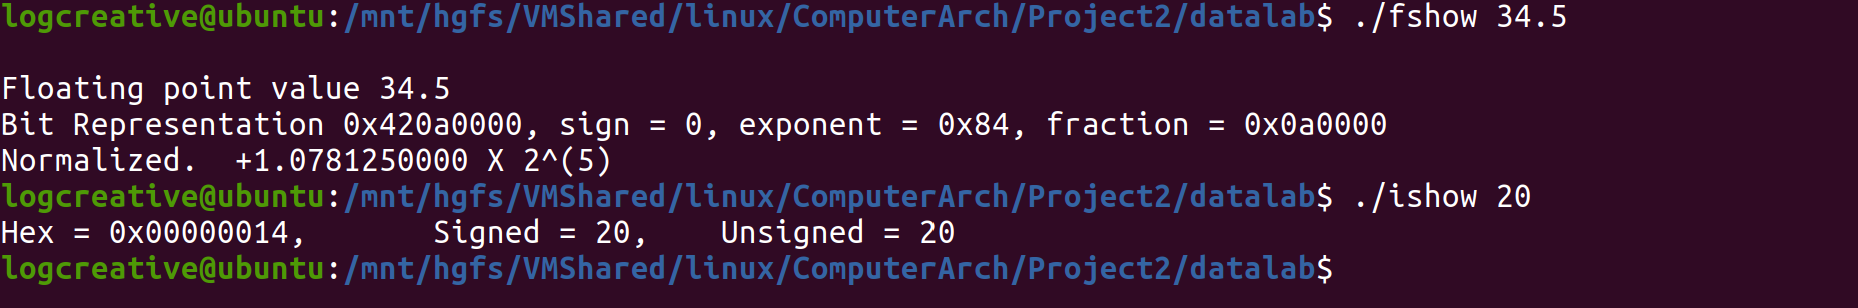
\includegraphics[width=0.8\textwidth]{showf.png}

    通过了检查测试,并得到了全部分数:

    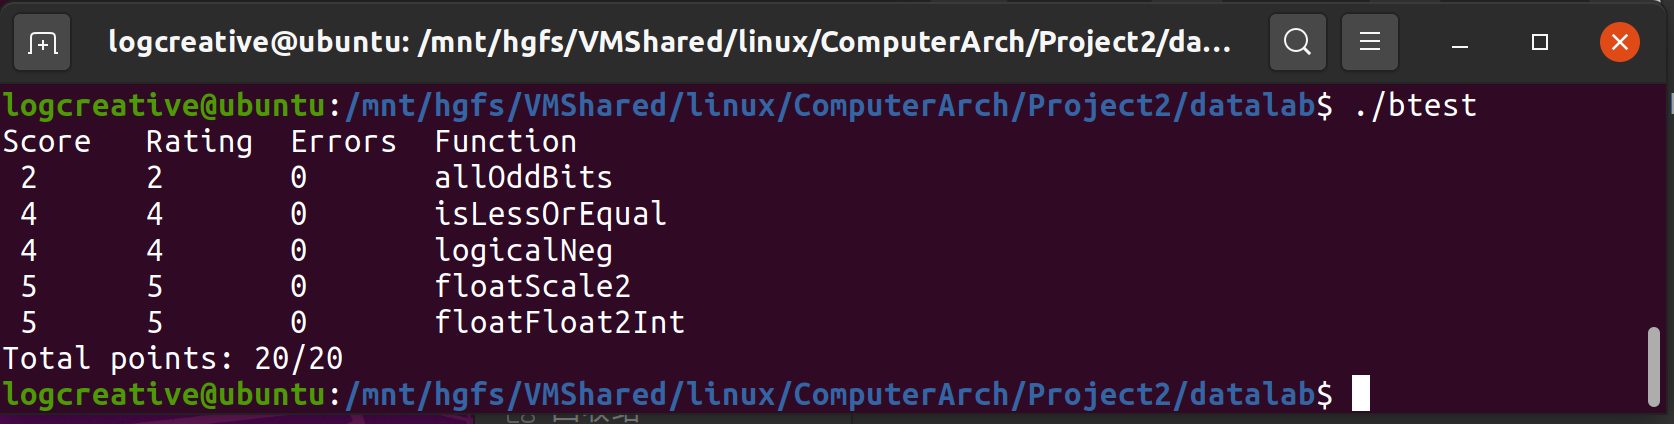
\includegraphics[width=0.8\textwidth]{score.png}

    \fname{bits.c}

    \inputminted[breaklines,autogobble,frame=lines,framesep=2mm,fontsize=\scriptsize]{c}{../datalab/bits.c}


\end{problems}


\end{document}
